\newpage
\renewcommand{\TheTitle}{Hybrid Woodcock-delta Tracking Schemes Using a Track-Length Estimator}
\renewcommand{\TheAuthors}{Joanna Piper Morgan,
  Ilham Variansyah,
  Kayla B. Clements,
  Todd S. Palmer,
  Kyle E. Niemeyer}

\renewcommand{\TheAddress}{%
In preparation for submission to\\
\textit{Journal of Computational and Theoretical Transport}
}

\PaperHeader{\TheTitle}{\TheAuthors}{\TheAddress}

\chapter{\TheTitle}
\label{chap:delta_tracking_paper}

\epigraphhead[10]{\singlespacing
    \epigraph{
        I would have really liked just doing laundry and taxes with you.
    }
    {Waymond Wang---Everything Everywhere All at Once}
}

%%% Write text for abstract
%%% Most text modifying commands will work in abstract

\section*{Abstract}

Woodcock-Delta tracking is a common alternative to the more popular surface tracking technique where the largest cross-section at a given energy in the whole problem is used to sample a distance to collision at any point.
This process forces extra nonphysical collisions so it is paired with a rejection sample to determine real events from virtual or phantom events.
Traditional implementations of Woodcock-delta tracking preclude the use of a track (or path-) length estimator for scalar flux tallies and are forced to use the normally higher-variant collision estimator instead.
There is no mathematical reason why the track-length estimator cannot be used in conjunction with Woodcock-delta tracking only implementation issues. 
In this work we take advantage of that to produce a Woodcock-delta tracking algorithm which tallies fluxes to a structured rectilinear mesh using the track-length estimator.
This development more readily enables hybrid surface-delta tracking algorithms as the track-length tally can be used everywhere for scalar flux estimation regardless of which tracking algorithm a particle is using.
We use this when developing a novel hybrid-in-energy method where Woodcock-delta tracking is used in high energies (where mean free paths are long) and surface tracking below that (starting at the neutron resonances) as well as a previously defined hybrid-in-material method.
We verify that delta tracking algorithms we consider can be used in conjunction with continuously moving surfaces.
We benchmark these methods showing figures of merit on four time-dependent problems: two multi-group and two continuous-energy.
Woodcock-delta tracking with a track-length tally showed modest improvements to figures of merit as compared to traditional delta tracking with a collision estimator and surface tracking with a track-length estimator (\num{1.5}$\times$--\num{2.5}$\times$) and significant improvements (\num{7}$\times$--\num{11}$\times$) when using the hybrid-in-energy method.

\section{Introduction}

% general introduction
Predicting the neutron distribution in space, energy and time is important when modeling inertial confinement fusion systems, pulsed neutron sources, and nuclear criticality safety experiments, among other systems.
The behavior of neutrons can be modeled with a Monte Carlo simulation, where particles with statistical importance are created and transported to produce a particle history \cite{lewis_computational_1984}. 
The path of a particle and the specific set of events that occur within its history are governed by pseudo-random numbers, known probabilities (for example, from material data), and known geometries. Data about how
particles move and/or interact with the system are tallied to compute parameters of interest with an associated statistical error from the Monte Carlo process.

There are two common methods used to sample the random walk in a Monte Carlo neutron transport algorithm: surface tracking \cite{lewis_computational_1984} and Woodcock-delta tracking \cite{woodcock_techniques_1965}.
These two tracking algorithms have complementary performance bottlenecks, for a certain class of problems, a hybrid method may allow for greater performance than either approach used individually.
For example: traditional implementations of Woodcock-delta tracking preclude evaluating quantities of interest with a track-length estimator instead opting for a collision estimator may be used, whereas, surface tracking has no such restrictions.
The track-length estimator usually provides a better estimate of quantities of interest (see section \ref{sec:tracking_algs_and_est}).
On the hand, surface tracking requires potentially complicated geometric operations whereas Woodcock-Delta tracking does not.
Which method to use is often problem dependent.

% cite previous M&C paper

Previous work into delta-surface tracking on a structured mesh has shown good performance for problems with complex arrangements of optically-thin materials\cite{morgan2023delta}.
Making material-based decisions about when to do delta and surface tracking has also been explored and implemented in production Monte Carlo codes \cite{leppanen_development_2013conf, leppanen_2010_burnup, richards_monk_2015}.
We extend the idea of \textit{tracking} on a structured mesh to full Woodcock-delta tracking (eliminating the distance to surface check) and \textit{tallying} to a structured mesh allowing the use of a track-length estimator for estimations of scalar flux.
% MC/DC introduction

In this work we describe, verify, and evaluate the performance of a delta tracking algorithm that allows the use of a track-length estimator on a structured tally mesh.
We then use this approach in two hybrid delta tracking schemes: one in which the choice tracking algorithm is based on material region, and another scheme based on the particle energy.
We implement this work in Monte Carlo Dynamic Code (MC/DC), an open source Monte Carlo neutron transport application purpose-built to conduct rapid numerical methods development, specifically for time-dependent problems \cite{morgan_monte_2024}.
We compute figures of merit for four computationally difficult benchmark problems including a stuck rod accident simulation of a continuous energy version of the C5G7 geometry, and runtime results for a whole CPU node (2X Intel x86 Xeon Sapphire Rapids) and a whole GPU Node (4X Nvidia Tesla V100).

This work is novel as it is the first published usage of a track-length estimator for scalar flux estimation with full Woodcock-delta tracking, the first usage of Woodcock-delta tracking in conjunction with continuously moving surfaces (implemented in MC/DC \cite{variansyah_2023_highfidelity}), and the first time a hybrid delta tracking method has been based on the energy of a given particle.
The quantities of interest in this work are estimates of scalar flux and not full reaction rate densities for all particle material interactions.
While this does limit the generally applicability of these methods, scalar flux is a necessary quantity for hybrid methods, and other uses.
Indeed for deterministic method if scalar flux is ascertained the problem is considered solved.


\section{Tracking Algorithms and Estimators}
\label{sec:tracking_algs_and_est}

% Surface tracking
To track the movement of neutrons within a system and, one of two tracking (or sampling) methods are employed. 
The first is surface tracking described in algorithm \ref{alg:surface}. 
For a particle in material $m$, a distance to collision is sample from a cumulative probability distribution function by
\begin{equation}
    d_{\text{collision}} = \frac{-\ln(\xi)}{\Sigma_{t,m}} \; ,
\end{equation}
where $\Sigma_{t,m}$ [\SI{}{\per\centi\meter}] is the macroscopic total cross section of the $m$-th material and $\xi$ is a pseudo-random number between zero and one.

This sampling of the cumulative probability distribution function will only hold true while the material is homogeneous.
So if the distance to collision is beyond a material interface in a system with multiple materials, the particle must be stopped at that interface surface and a new distance to collision must be calculated with with the new material's $\Sigma_{t,m}$.
This approach is an unbiased way of dealing with the sampling of distance to collision in a heterogeneous medium.
In a standard surface tracking algorithm this involves computing both a distance to collision ($d_{\text{collision}}$) and a distance to the nearest surface along the particle's direction of travel ($d_{\text{surface}}$).
The smaller of these two distances determines which event happens to the particle - a collision or a surface-crossing.
After or while the particle is moving, tallies can be accumulated to compute quantities of interest.
If a collision occurs, more sampling and operations can be done (e.g., isotropically scatter a particle).
If the particle is still alive at the end, the algorithm is repeated.
The distance to nearest surface computation can become quite expensive as geometries grow in complexity (e.g., complex CSG geometries or CAD based surfaces).
Surface tracking is at the heart of many modern Monte Carlo neutron transport applications, including MCNP \cite{MCNP_RisingArmstrongEtAl}, Shift \cite{hamilton_continuous-energy_2019, pandya_implementation_2016}, MONK/MCBEND \cite{richards_monk_2015}, and OpenMC \cite{romano_openmc_2015}.


\begin{algorithm}
\begin{algorithmic}[1]
    \State $m =$ lookup material in current particle location

    \State $\Sigma_{t,m} =$ look up total macroscopic cross section of material $m$ 

    \While{particle is alive}
    
        \State $d_{\text{collision}} = -\ln{\xi} / \Sigma_{t,m} $
        
        \State $d_{\text{surface}} =$ compute distance to nearest surface along particle direction of travel

        \If{$d_{\text{collision}} < d_{\text{surface}}$}

                \State $d = d_{\text{collision}}$
                
                \State sample collision type
                
                \State carry out collision
                
            \Else 

                \State $d = d_{\text{surface}}$
        
                \State move particle to surface
    
                \State $m =$ lookup material on the other side of the surface
    
                \State $\Sigma_{t,m} =$ look up total macroscopic cross section of material $m$ 
    
                \If {surface is a boundary}
    
                    \State implement boundary condition
    
                \EndIf
        \EndIf
        \State score track-lengths to tally bins
    \EndWhile
    \caption{A generic surface tracking algorithm.}
    \label{alg:surface}
\end{algorithmic}
\end{algorithm}


Delta tracking is the next most common tracking approach and is shown in algorithm \ref{alg:trad}.
It starts by pre-processing a \textit{majorant} macroscopic cross-section
\begin{equation}
    \maj(E) = \max\left({\Sigma_{t,1}(E), \Sigma_{t,2}(E) \dots \Sigma_{t,m}(E) \dots \Sigma_{t,M}(E)}\right)
\end{equation}
such that it is the largest cross section at any given point in any material in the problem.
The algorithm to compute the majorant cross-section for nuclides on a non-unified energy grid currently implemented in MC/DC is in appendix \ref{app:majorant}.
Figure \ref{fig:majorant_c5ce} at right shows a macroscopic majorant cross section for a typical pressurized water reactor.
When delta tracking the distance to collision is always computed with the majorant,
\begin{equation}
    _{\text{collision}} = \frac{-\ln{\xi}}{\maj} \; ,
\end{equation}
ignoring surface crossing events.
However, this sampling forces extra collisions that do not physically exist; using the majorant generates the smallest distance to collision. Delta tracking algorithms use a rejection sampling to determine if the sampled collision event was \textit{real} or a \textit{virtual} (\textit{phantom}) collision.
At the particle's current location, the true material region of the is be identified to compute $\Sigma_{t,m}$.
If 
\begin{equation}
    \xi > \frac{\Sigma_{t,m}}{\maj} \; ,
\end{equation}
where $\xi$ is a new random number, the collision did not physically occur, is rejected, and the particle can be left alive on it's current direction of travel and energy.
From here the process is the same as before: tallies are accumulated, real collision physics are carried out when appropriate, and the algorithm continues as long as the particle is still alive.

\begin{figure}
    \centering
    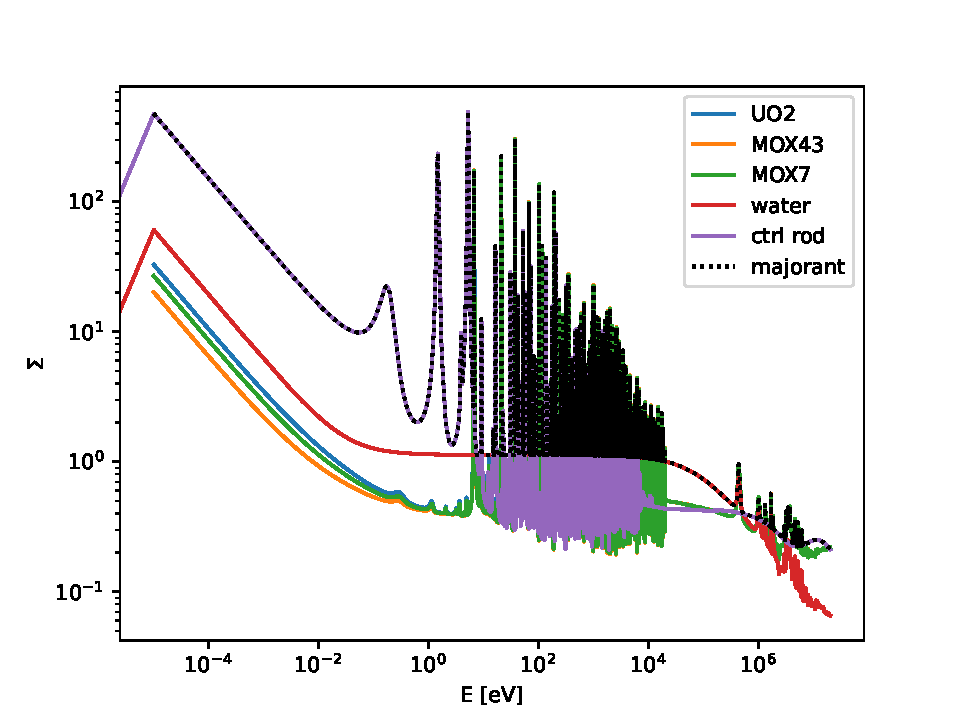
\includegraphics[width=0.75\textwidth]{figures/delta_figs/macro_majorant_c5ce.pdf}
    \caption{Continuous energy macroscopic majorant cross-section ($\maj$) for the continuous energy version of C5G7 PWR described in appendix \ref{app:c5ce_mat}.}
    \label{fig:majorant_c5ce}
\end{figure}

When undergoing delta tracking some way to kill or reflect particles on vacuum or reflecting boundary conditions respectively is needed.
In a code that already implements surface tracking, the functionality to track distances to specific surfaces will already exist.
So it is natural when undergoing delta tracking to only compare distances to boundary surfaces exclusively.
Boundary surfaces are often planar, making the computation trivial and cheap.
%This is similar to other methods currently under development in OpenMC.

\begin{algorithm}
\begin{algorithmic}[1]
    \While{particle is alive}
        \State $d_{\text{collision}} = -\ln{\xi} / \maj $
        \State $d_{\text{boundary}} =$ compute distance to boundary
        
        \If {$d_{\text{collision}} < d_{\text{boundary}}$}
            \State $m =$ lookup material in current particle location
            \State $\Sigma_{t} =$ look up total macroscopic cross section of material $m$ 

            \If  {$\xi < \Sigma_{t} / \maj$}
                \State collision is rejected

            \Else 
                \State collision is accepted
                \State tally $1/\Sigma_t$ to bin at particles current location
                \State determine collision type 
                \State carry out collision
            \EndIf
         \Else 
            \State move particle to boundary
            \State implement boundary condition
        \EndIf
    \EndWhile
    \caption{Woodcock-delta tracking in MC/DC. Notably we are still surface tracking to boundaries.}
    \label{alg:trad}
\end{algorithmic}
\end{algorithm}

An added complication when using the Woodcock-delta tracking method is restricting what type of tallies can be efficiently scored.
There are many so called estimators that can be used to indicate quantities of interest (often scalar flux) by tallying events that occur within a given region of phase space.
The two common estimators are the collision estimator and the the track (or path) length estimator.
Often tallies are scored to bins on a structured mesh grid overlying the surfaces and material regions that a Monte Carlo simulations uses to conduct actual transport operations.
The track-length estimator is,
\begin{equation}
    \label{eq:pathlength}
    \hat{\phi}_n = \sum_{i=1}^{I}p_i \; ,
\end{equation}
where $\hat{\phi}_n$ is the integrated scalar flux over given mesh cell $p$ is the track-length of particle $i$ passing through mesh cell $n$.
The collision estimator is,
\begin{equation}
    \label{eq:collision}
    \hat{\phi}_n = \sum_{i=i}^{I} \frac{1}{\Sigma_{t,n}} \;.
\end{equation}
The collision estimator will often produce a more variant solution as compared to other estimators for tallies where $\Sigma_{t,m}$ is small (optically thin, less dense materials) and will never tally anything into a void region.
On the other hand the track-length estimator will always tally into every mesh bin as particles moves.
Meaning, undermost problem regimes, more information will be scored, which will result in a lower-variant tally for the same number of particles.

Both of the estimators in Eqs. \ref{eq:collision} and \ref{eq:pathlength} are only for flux integrals, where response functions are one.
Other response functions for other reaction rates (e.g., fission rate density) will require the knowledge of the macroscopic cross section of that operation in a given location.
In this work we limit ourselves to flux integrals only.
Thus we also only enable these schemes for fixed source problems and leave k-eigenvalue calculations for future work.
This does currently limit the more general applicability of the methods we implement, tho future work may extend these methods to allow for the computation of these perimeters.
We discuss this further in section \ref{disucssions}.

Delta tracking algorithms are implemented in many production Monte Carlo neutron transport applications including Serpent \cite{leppanen_2010_burnup, leppanen_use_2017, leppanen_development_2013, leppanen_2015_serpent}, MONK/MCBEND \cite{richards_monk_2015}, and GUARDYAN \cite{molnar_gpu_based_2019}.
Notably, the MONK Monte Carlo neutron transport code is the direct successor to the GEM code where Woodcock et. al first implemented Woodcock-delta tracking \cite{woodcock_techniques_1965}.
There are other weighted Woodcock-delta tracking algorithms, in this work we explore variants of non-weighted version \cite{molnar_variance_2018, morgan_weighted-delta-tracking_2015}.

% what other codes do and how this work is novel
Modern transport applications often choose one-or-the other tracking algorithm and optimize from there. However, either method of sampling the probability distribution functions can hold valid for the same system in the same simulation even at the same location in phase space.
Serpent Monte Carlo code establishes regions of delta tracking and surface tracking based on the ratio between the ratio of $\Sigma_{t,m}$ and $\maj$.
MONK/MCBEND support material regions inside of which delta tracking is implemented (called Hole geometries) where surface tracking is implemented else where.
Ongoing developments in OpenMC and MCNP will introduce similar delta tracking algorithms for 
Publications indicate that no other Monte Carlo neutron transport application currently supports the use of any track-length estimator within a region undergoing Woodcock-delta tracking.


\section{Hybrid Delta Tracking Schemes}

In this section we introduce and verify the voxilized tally structure that allows MC/DC to use a track-length estimator while Woodcock-delta sampling.
We also introduce two hybrid surface-delta tracking schemes we implement in time-dependent transport with moving surfaces in MC/DC.
The first is a region based delta tracking method which has been implemented before in other production Monte Carlo neutron transport applications.
The second and novel method where delta tracking is used in high-energies above neutron cross-section resonances, where total cross sections are often similar to the majorant, and track-lengths are long relative to nominal system dimensions.


\subsection{Voxelized Tallies}
\label{sec:voxtallies}

Traditional Woodcock-delta tracking algorithms do not keep track of what material or physical mesh cell a given particle occupies at any moment in transport.
Conventional wisdom dictates that repeatedly conducting lookups of locations, cross sections, and tally bin indices while delta-tracking would be prohibitively costly and eliminate any boon to performance that system homogenization gave.
It follows that Woodcock-delta tracking precludes use of a track-length estimator for quantities of interest.
Crucially there is nothing \textit{mathematically} preventing the use of a track-length estimator with Woodcock-delta tracking, only engineering issues.
Furthermore if all that are needed to quantify a given problem is the total integral flux no such extra cross section lookups are needed.
Only an identification of the track-length and bin to accumulate.
This forms the underlying assumptions that are used in this work.

\begin{figure}[!htb]
  \centering
  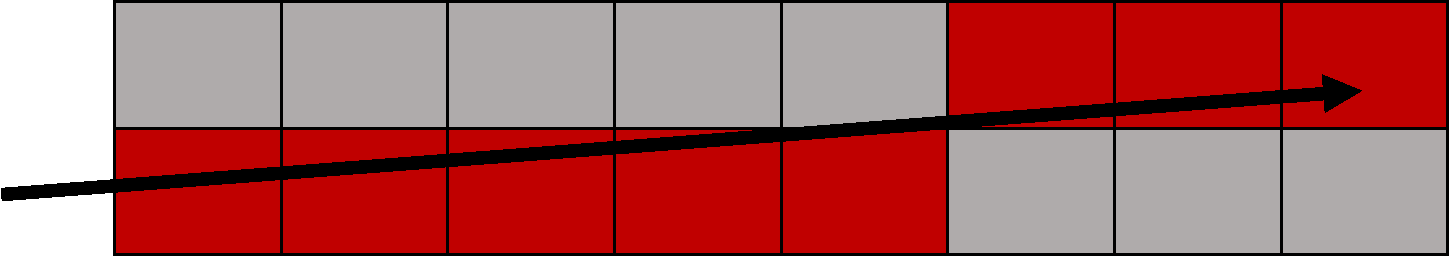
\includegraphics[width=\textwidth]{figures/delta_figs/tally_ray.pdf}
  \caption{A particle tallying to multiple tally mesh bins (shown in red). Implemented as a single operation for both surface and Woodcock-delta tracking in MC/DC.}
  \label{fig:tally_ray}
\end{figure}

MC/DC v0.11.1 \cite{morgan_monte_2024} has an optimized tally algorithm where track-lengths to multiple structured mesh cells (which we call voxels
\footnote{\textit{voxel} is the 3D analog to a pixel, here we mean it as a cube mesh bin to tally into}
)are scored in a single operation.
This algorithm is based on a sweeping method where the initial state (mesh cell index, exact ($x$, $y$, $z$) position, direction of travel, speed, and particle clock) are known, as is the distance to the next event.
The particle is then swept from voxel to voxel, tallying the exact track-length traveled in a given voxel along the way.
Figure \ref{fig:tally_ray} shows a hypothetical particle track and the mesh bins to be tallied to (in red) in a single operation.
In MC/DC's normal algorithm this is done even before moving a particle to an event while surface tracking.

In this work, we used this voxlized tally scheme when undergoing Woodcock-delta tracking.
Even if a particle collision is rejected that particle still physically moved to the location that was sampled, allowing the use of the track-length estimator.
In this scheme the distance tallied is always the distance sampled with the majorant, baring census crossings or distance to boundary events.

To verify that MC/DC's voxelized track tallies with delta tracking both converges to the correct solution and at the correct rate we use four anaclitic based benchmark problems.
We compare the error from integral quantities of interest to a reference solution then plot the error as a function of increasing particle count.
The convergence rate should be the standard Monte Carlo convergence rate of $N^{-1/2}$.
Our verification problems are
\begin{itemize}
    \item AZURV1 time-dependent benchmark both super and sub critical (figure \ref{fig:azurv1}) \cite{ganapol_homogeneous_2001};
    \item A time-dependent infinite pin cell using the 371 group SHEM cross sections (figure \ref{fig:shem}) \cite{hfaiedh_2005_shem}; and 
    \item Reed's Problem (figure \ref{fig:reeds}) \cite{reed_difference_1971};
    \item A purely absorbing slab (figure \ref{fig:abs_slab}).
\end{itemize}
\begin{figure}
  \centering
  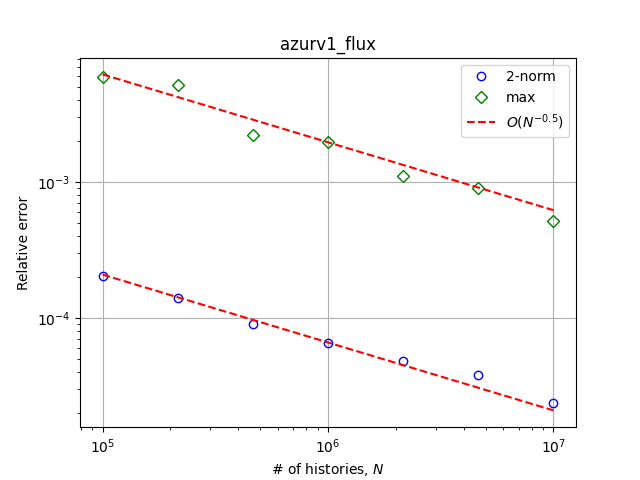
\includegraphics[width=0.32\linewidth]{figures/delta_figs/verification/azurv1/azurv1_flux.png}
  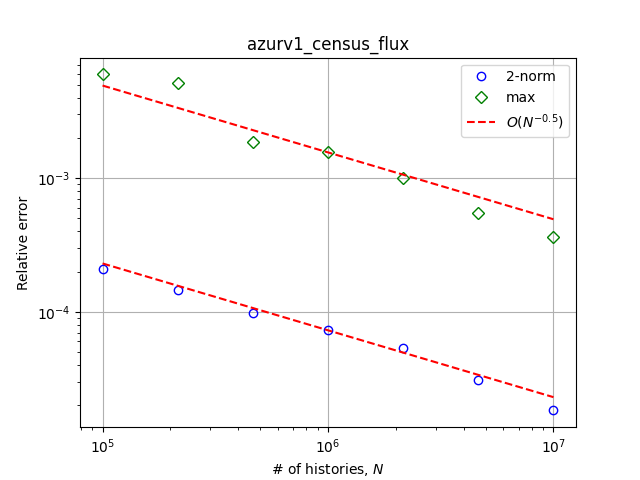
\includegraphics[width=0.32\linewidth]{figures/delta_figs/verification/azurv1/azurv1_census_flux.png}
  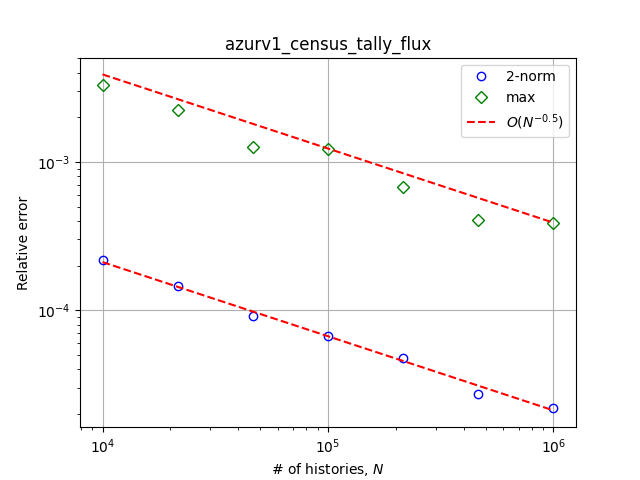
\includegraphics[width=0.32\linewidth]{figures/delta_figs/verification/azurv1/azurv1_census_tally_flux.png}
  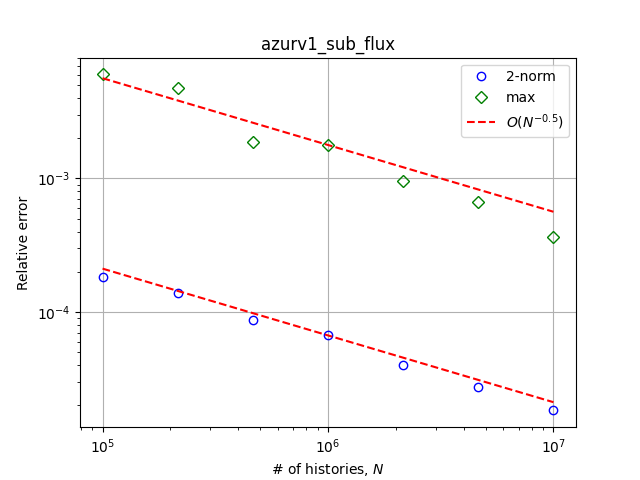
\includegraphics[width=0.32\linewidth]{figures/delta_figs/verification/azurv1/azurv1_sub_flux.png}
  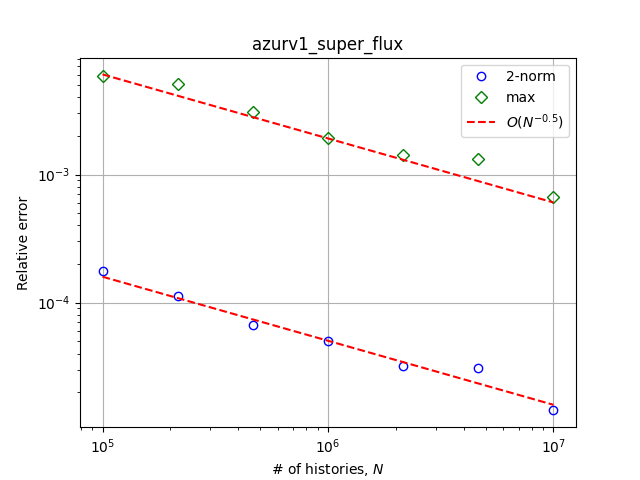
\includegraphics[width=0.32\linewidth]{figures/delta_figs/verification/azurv1/azurv1_super_flux.png}
  \caption{Convergence rate verification of AZURV1 \cite{ganapol_homogeneous_2001} }
  \label{fig:azurv1}
\end{figure}
\begin{figure}
  \centering
  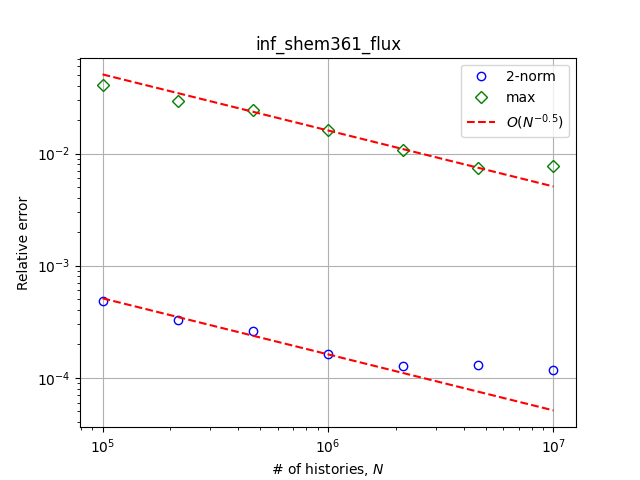
\includegraphics[width=0.32\linewidth]{figures/delta_figs/verification/shem/inf_shem361_flux.png}
  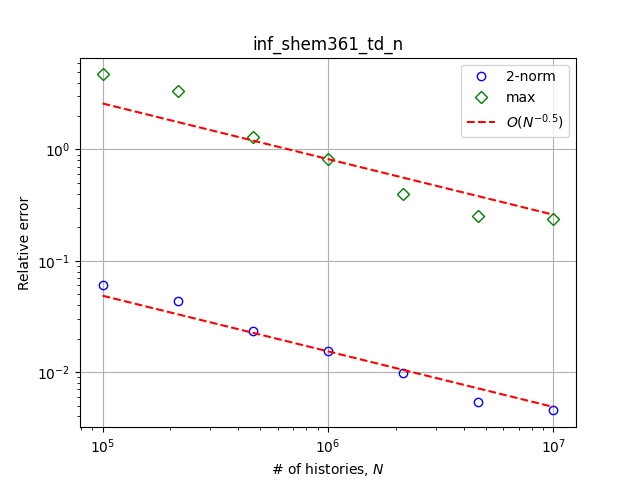
\includegraphics[width=0.32\linewidth]{figures/delta_figs/verification/shem/inf_shem361_td_n.png}
  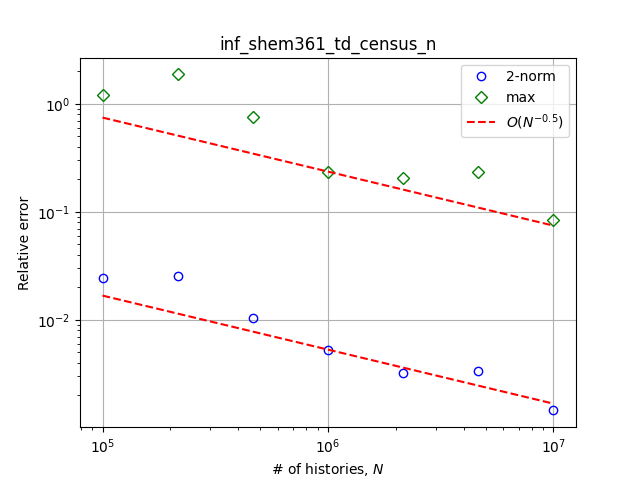
\includegraphics[width=0.32\linewidth]{figures/delta_figs/verification/shem/inf_shem361_td_census_n.png}
  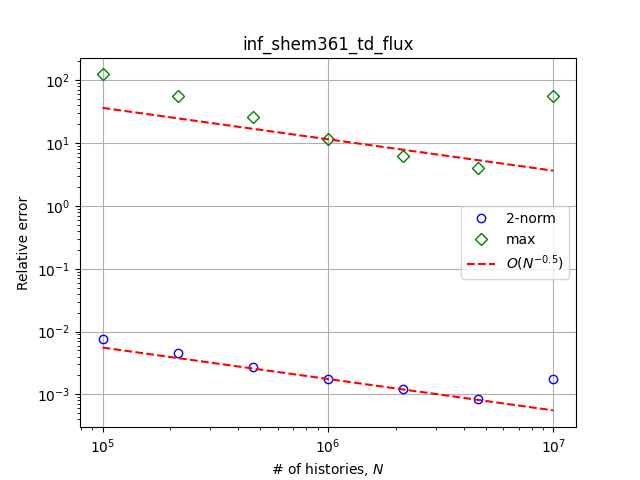
\includegraphics[width=0.32\linewidth]{figures/delta_figs/verification/shem/inf_shem361_td_flux.png}
  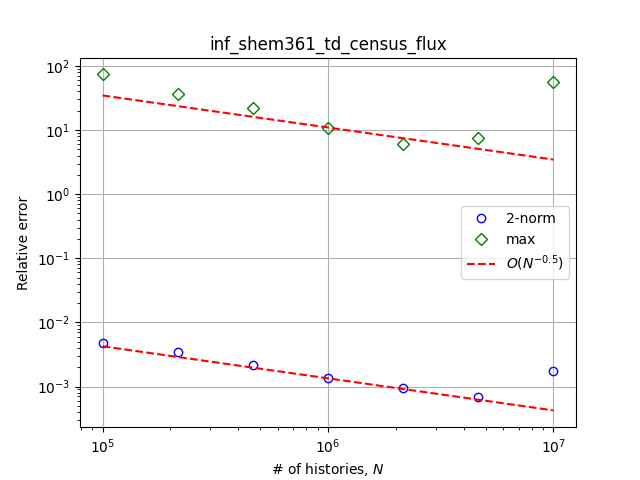
\includegraphics[width=0.32\linewidth]{figures/delta_figs/verification/shem/inf_shem361_td_census_flux.png}
  \caption{Convergence rate of an infinite pin using the SHEM 361 group cross section library \cite{hfaiedh_2005_shem}}
  \label{fig:shem}
\end{figure}
\begin{figure}
  \centering
  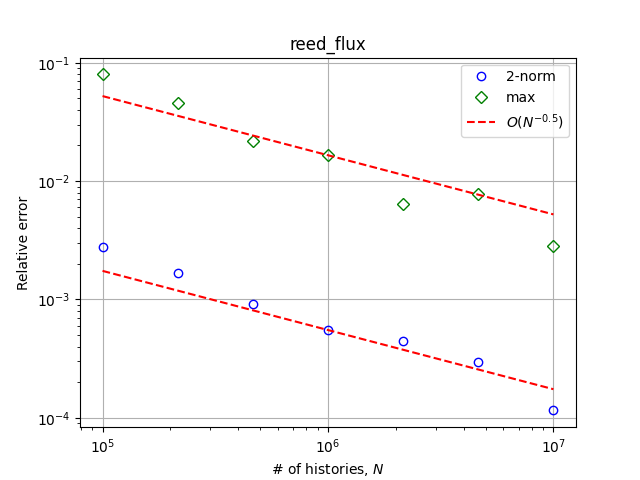
\includegraphics[scale=0.75]{figures/delta_figs/verification/reed/reed_flux.png}
  \caption{Convergence rate of flux from Reed's problem \cite{reed_difference_1971}}
  \label{fig:reeds}
\end{figure}
\begin{figure}
    \centering
    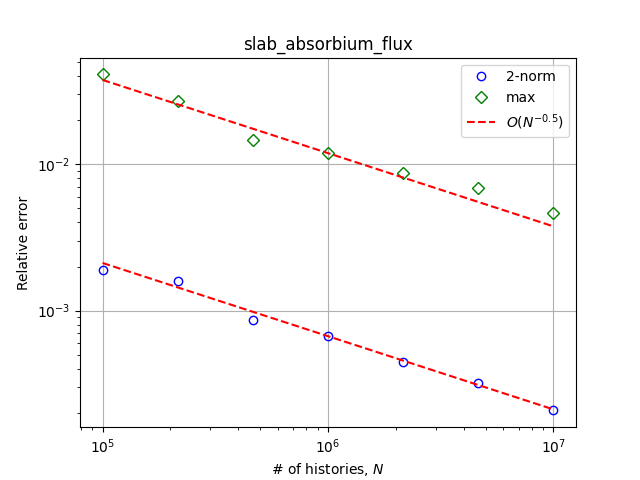
\includegraphics[width=0.75\linewidth]{figures/delta_figs/verification/abs_slab/slab_absorbium_flux.png}
    \caption{Convergence rate of QOIs for a purely absorbing slab wall problem}
    \label{fig:abs_slab}
\end{figure}

All verification simulations show the $N^{-1/2}$ convergence rate expected for Monte Carlo results.
This verifies that we are getting the expected results with voxelized Woodcock-delta tracking.


\subsection{Hybrid-In-Material}
\label{sec:material_exc}


The first hybrid method we implement in MC/DC is a material or region based decision on weather to us surface or delta tracking we call ``hybrid-in-material".
Each particle is given an additional flag declaring which transport algorithm it is using to sample a distance to next event.
At the beginning of the \texttt{determine\_next\_event} function the tracking flag will be set to \texttt{true} if the particle is in a material region declared by the user to undergo delta tracking or \texttt{false} if in a region where delta tracking should not be used. 
This is similar to in Serpent2's algorithm however our voxelized tally structure allows us to use track-length estimators in all regions not just those undergoing surface tracking.
Also Serpent2's algorithm makes automatic decisions about where to surface and delta track based off a user supplied cut off value \cite{leppanen_development_2013} whereas we leave it as user option for now.


\begin{figure}
    \centering
    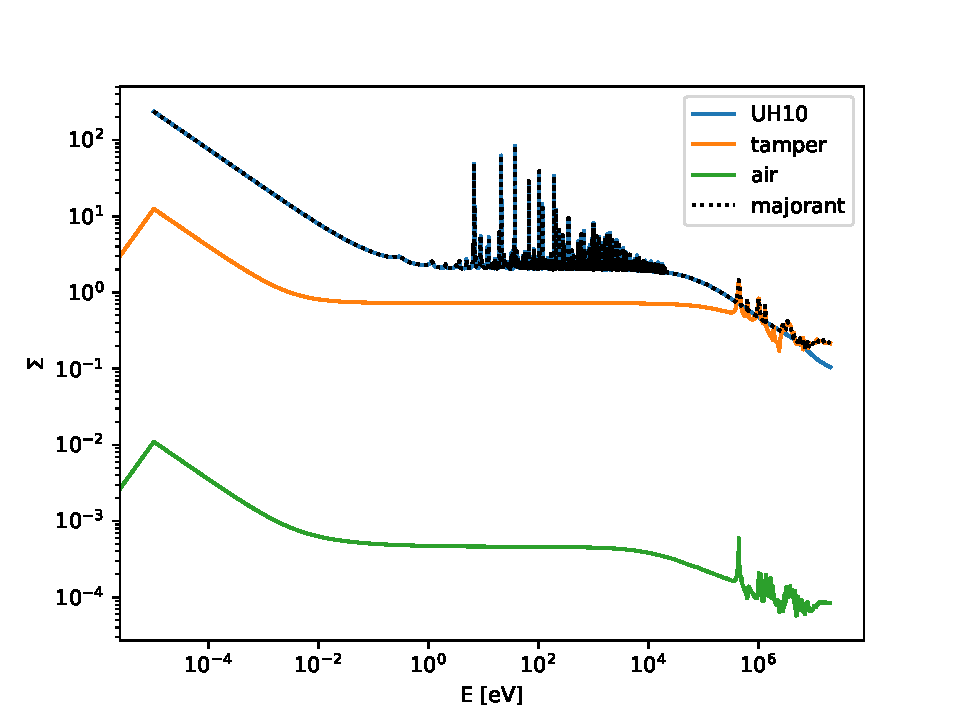
\includegraphics[width=0.75\textwidth]{figures/delta_figs/macro_majorant_dragon.pdf}
    \caption{Continuous energy macroscopic majorant cross-section ($\maj$) for the Dragon burst problem.}
    \label{fig:majorant_dragon}
\end{figure}

Conventional wisdom dictates that delta tracking should not be used in systems with strong localized absorbers as the majorant will be governed by cross sections much larger then others in the system.
Figure \ref{fig:majorant_dragon} shows the cross section information for the Dragon burst problem we describe in section \ref{sec:benchmarks}.
Conventional wisdom would suggest that this is a simulation that does not warrant Woodcock-delta tracking.
This simulation contains three materials, two of which (the fuel and tamper) have similar cross sections over all energies clumped together.
However the cross sections modeling air are over four orders of magnitude under cross sections describing the fuel and tamper.
This means in the air, particles will get stuck in the rejection sampling loop having phantom collision after phantom collision and statistically rarely complete a particle history.
Furthermore for classical delta tracking (where only a collision estimator can be used) the tallies in the air will be highly variant as there will be statistically few collisions taking place.
Using surface tracking in the air and delta tracking in the material may give a performance boost in this problem.

\subsection{Hybrid-In-Energy}
\label{sec:cutoff}

The second hybrid method we call ``hybrid-in-energy", and is a decision to do delta tracking above a given user-defined energy and conduct surface tracking below.
For neutrons, high energies (or speeds) are characterized by relatively long mean free paths (small cross sections) as they are physically going too fast to interact with anything.
Delta tracking generally does better under these conditions compared to surface tracking as surface tracking would get stuck moving particles from region to region whereas delta tracking can stream particles through the whole problem.
Furthermore at higher energies in many systems the majorant will more closely match the cross sections of materials in alleviating issues with the rejection sampling loop.

For example consider a continuous energy version of the C5G7 benchmark reactor geometry \cite{jia_hou_oecdnea_2017}.
The material composition is given by table \ref{tab:c5ce} in appendix \ref{app:c5ce_mat}.
Figure \ref{fig:majorant_c5ce} shows the macroscopic material cross-sections for the 7 material reactor with the majorant in black.
Around \SI{10}{\kilo\electronvolt} the neutron resonances end and the problem can be considered high energy.

If using delta tracking for this whole problem neutrons will get stuck in resonance frequencies where the rejection sampling loop will be called too much degrading the performance of delta tracking.
Therefore it would be ideal to delta track above \SI{50}{\kilo\electronvolt} (as to completely avoid neutron resonances) and surface track under that threshold.

\subsection{Implementation in MC/DC}
\label{sec:implementation}

Monte Carlo Dynamic Code is purpose built to implement and test time-dependent Monte Carlo novel numerical methods at scale \cite{morgan_2025_monte}.
It uses a novel for the field development structure where Python scripted compute kernels are compiled via the Numba compiler to run on CPUs and with the Harmonize GPU runtime manager to run on GPUs.

MC/DC allowed us to rapidly experiment with these methods at scale on both CPUs and GPUs on time-dependent problems of interest.
Delta tracking methods can be easy to implement in a code that already conducts surface tracking. 
Generally to implement delta tracking in a code that already implements surface tracking add are:
\begin{enumerate}
    \item Pre-process functions to generate a majorant (MC/DC's implementation is in \ref{app:majorant});
    \item \texttt{if} statements in \texttt{distance\_to\_next\_event} functions to compute relevant distances;
    \item Functions to implement boundary conditions when in delta tracking mode; and
    \item Elevate delta tracking options to the input deck.
\end{enumerate}
Our implementation added about \num{450} lines of code, of which half was to produce various types of majorants (an example can be found in \ref{app:majorant}). 
Only about \num{200} lines of code where required in the compute kernels themselves to implement delta tracking in MC/DC.
This process was similar to implementing hybrid surface-delta tracking methods in MCATK \cite{morgan2023delta}.
This is also similar to current ongoing work in OpenMC.

We found the most complicated issue when implementing delta tracking in MC/DC to be the boundary conditions.
Surface tracking codes (like MC/DC) often enforce boundary conditions as a surface options, something to avoid when delta tracking.
Vacuum boundary conditions are simple as if or when a particle is determined to be out of the problem when looking for a cross section in the rejection sample particles are killed.
For reflecting surfaces we use a stripped down version of \texttt{distance\_to\_nearest\_surface} function in MCDC to compute distances to reflecting surfaces, if any.
Many reflecting boundary conditions including the ones we implement in our benchmark problems are imposed on planar surfaces, making the distance to boundary computation cheap.
In effect we are still surface tracking only to our reflecting boundary surfaces.


\section{Verification of Woodcock-Delta Tracking with Continuously Moving Surfaces}

To verify that Woodcock-delta tracking can be used in conjunction with the continuously moving surfaces in MC/DC we use the moving pellet regression test from MC/DC's test suite \cite{morgan_monte_2024}.
In it a rectangular fuel element which moves through a region with a small source.
As the pellet moves closer and farther from the source region the fission rate in the pellet changes.
Figure \ref{fig:moving_pellet} at left shows the fission reaction rate density at various points in time.
The outline of the pellet can be seen clearly.
These plots where produced using Woodcock delta tracking with a collision estimator and matched plots produced when using surface tracking with a collision estimator.

\begin{figure}
    \centering
    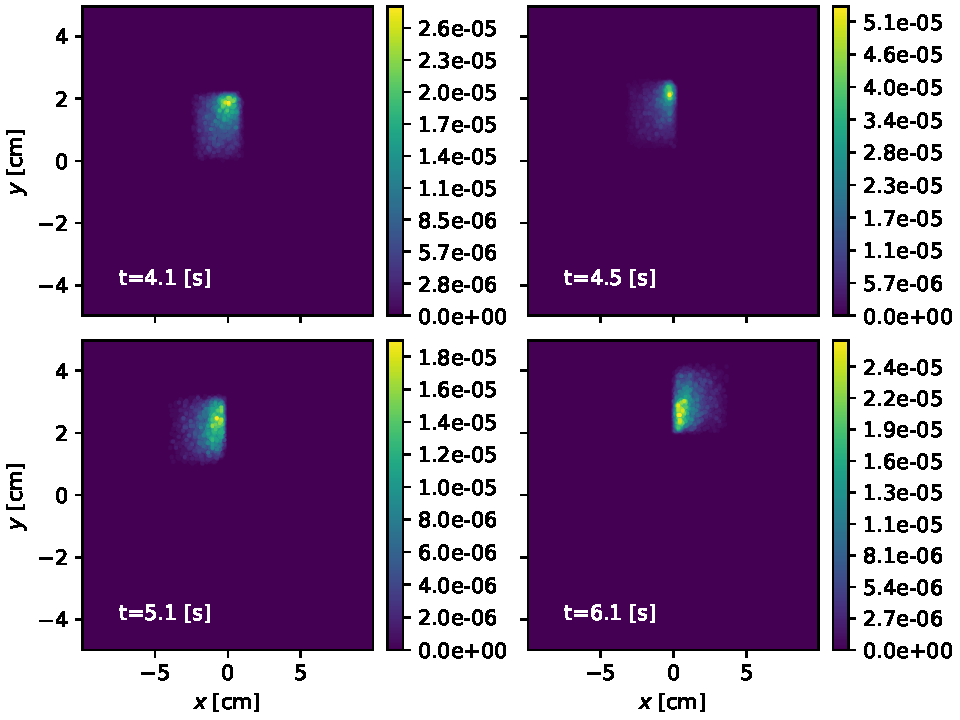
\includegraphics[width=0.49\linewidth]{figures/delta_figs/verification/moving_pellet_plot.pdf}
    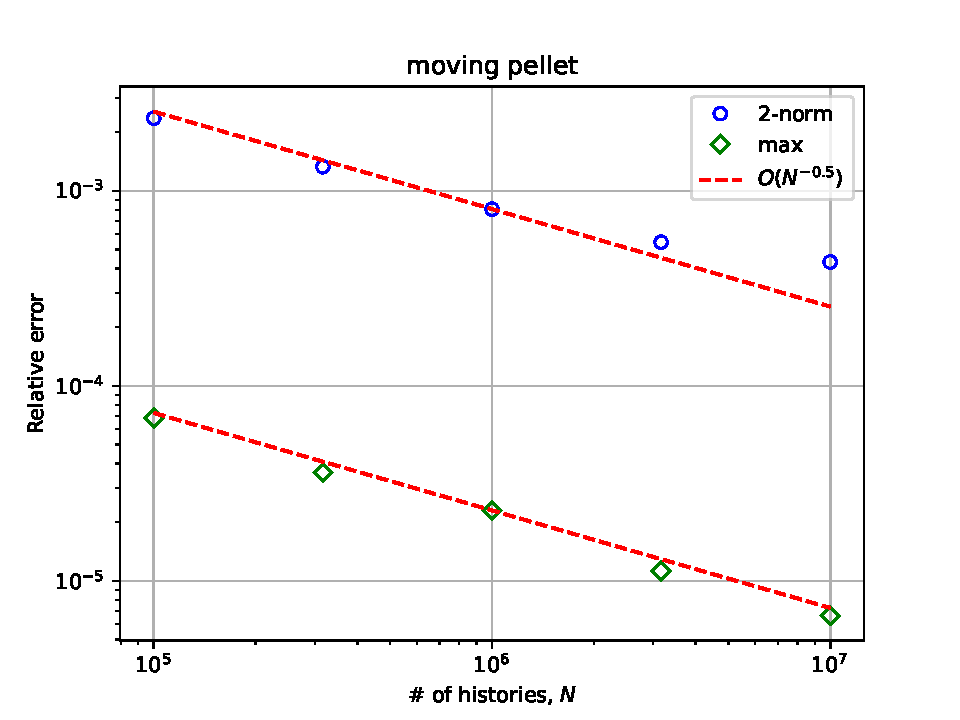
\includegraphics[width=0.49\linewidth]{figures/delta_figs/verification/moving_pellet.pdf}
    \caption{(left) Fission flux density at various points in time for the moving pellet problem, using Woodcock-delta tracking with a collision estimator (right) convergence between fluxes produced from surface and Woodcock-delta tracking both with the track-length estimator, showing $N^{-1/2}$ convergence rate.}
    \label{fig:moving_pellet}
\end{figure}

To further verify Woodcock delta tracking with continuous movement physics we regressively compare the flux solutions provided from traditional surface tracking and delta tracking with voxelized tallies at various particle counts.
We compute 
\begin{equation}
    \epsilon_N = ||\phi_N^{\text{surface}} - \phi_N^{\text{delta}} ||_2
\end{equation}
at every choice of $N$ particles.
We then compare the error of flux over particles to ensure the expected Monte Carlo convergence rate ($N^{-0.5}$).
Figure \ref{fig:moving_pellet} at right shows the error converging at the expected rate.
This regressively verifies that Woodcock-delta tracking can be used in conjunction with continuously moving surfaces.
We also produced this same plot for both tracking method using a collision estimator for both flux and fission tallies all of which matched the expect Monte Carlo convergence rate.

\section{Benchmark Problems}
\label{sec:benchmarks}

% vairiance reudciton and figure of merrit
The performance of a given Monte Carlo algorithm for a specified problem is a function of solver variance ($\sigma^2$, from the Monte Carlo process itself) and wall-clock runtime it takes to get that solution.
If a certain algorithm can forum a solution with low variance at fewer particles it may still yet be not considered as suitable as an algorithm that takes many many more particles to reach that statistical variance if it is too slow.
So a measurement must be used to take into account both the variance of a given solution and Figure of Merit (FOM) is one such measure. In this work we will use 
\begin{equation}
    FOM = \frac{1}{\hat{\sigma}^2 t_{wc}}
\end{equation}
where $\hat{\sigma}^2$ is the L$_{1}$ norm (over phase space) of the variance of the solution provided by the Monte Carlo solver and $t_{wc}$ is the wall clock runtime required to obtain that solution.

\begin{figure}
    \centering
    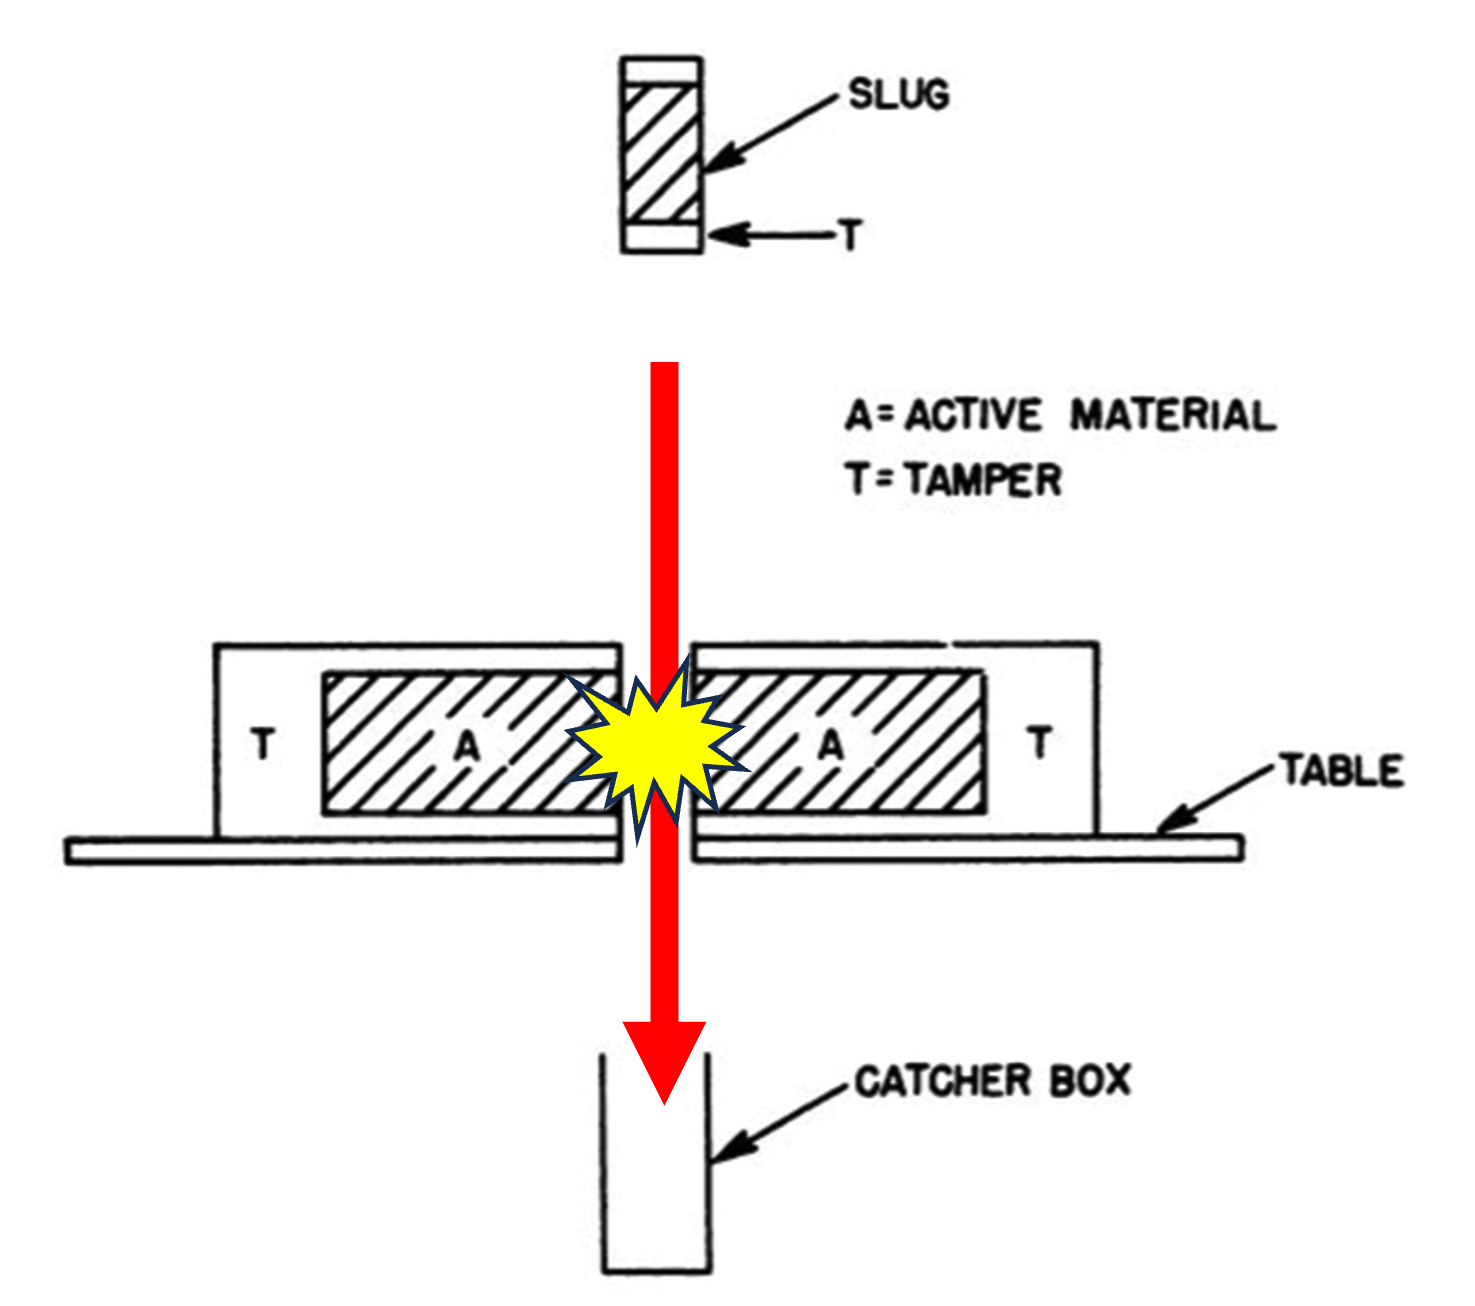
\includegraphics[width=0.48\linewidth]{figures/delta_figs/dragon.png}
    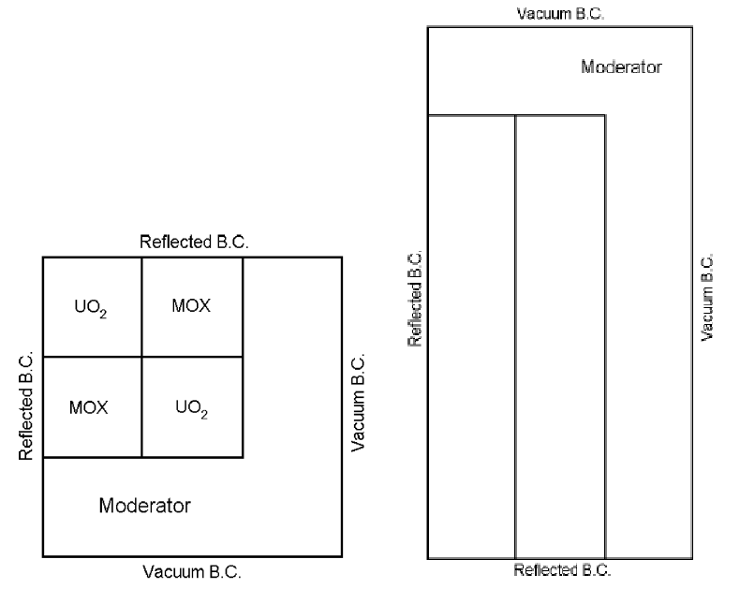
\includegraphics[width=0.48\linewidth]{figures/delta_figs/c5g7.png}
    \caption{Schematics (left) Dragon burst problem \cite{kimpland2021dragon} (right) C5G7 reactor quarter (via reflecting boundaries) \cite{jia_hou_oecdnea_2017}}
    \label{fig:schems}
\end{figure}

% the problems we run themselves
We use four fully time-dependent fixed source benchmark problems to compare the voxlized tally scheme and hybrid methods proposed in this work to surface tracking on CPU and GPU machines.
Two are multi-group, two are continuous energy.
Table \ref{table:benchmark_problems} summarizes the size (in both mesh and particle count) of each benchmark problem.
Some problems may not be suited for delta tracking methods but are used anyway here to show both correctness under physical problem dynamics (i.e., moving surface) and demonstrate algorithmic improvement in under highly exaggerated problem parameters.

\begin{table}[htb]
  \centering
  \begin{tabular}{@{}l c c c @{}} \toprule
    Problem & $N_{mesh}$ & $N_{particles}$ & Energy physics \\ \midrule
    Kobyashi & \num{120e3} & \num{1e10} & MG (1 group) \\
    Dragon Burst & \num{4.0e6} & \num{3e9} & Cont. E (3 materials) \\
    C5G7 & \num{3.9e6} & \num{1e7} & MG (7 groups) \\
    C5CE & \num{544e3} & \num{1e5} & Cont. E (7 materials) \\
    \bottomrule
  \end{tabular}
  \caption{time-dependent benchmark problems.} 
  \label{table:benchmark_problems} 
\end{table}

% koby intro
The first benchmark we consider is the time-dependent version of the Kobyashi problem \cite{Kobayashi2001} introduced by \cite{morgan_2025_monte}.
We run this problem with 10 batches with \num{1e9} particles per batch (\num{1e10} particles total) with traditional surface tracking, traditional delta tracking with a collision estimator, and a delta tracking using the voxelized tally method.
This problem contains two materials, a dense region (characterizing a solid), and a low density region modeled by air (characterizing a void) in a single energy group.
There are a 120k structured tally mesh cells in the $x$-$y$ plane and in time.

% acident intro
Figure \ref{fig:schems} at right shows the geometry for the next two simulations we consider based on the C5G7 benchmark problem \cite{jia_hou_oecdnea_2017}.
We model a four-phase accident where-in a pressurized light water reactor reactor is powering up by removing control rods.
Figure \ref{fig:c5g7} at left shows the normalized flux density as a function of time (produced from reactor point kinetics) and the four phases shaded as gray, green, red, and blue.
Phase one (shaded gray) starts with the reactor operating at steady state.
In phase two (shaded green) the control rods are removed from the reactor to power up to a new steady state.
Phase three (shaded red) begins when a bank of control rods gets stuck in the fully withdrawn position.
Towards the end of phase three the reactor sees a rapid spike in power that ends when at \SI{15}{\s} all the control rods are forced into the reactor ending the accident.
The fourth and final phase sees the reactor decaying in power as the delayed neutron population dies out.
Figure \ref{fig:c5g7} shows plots of flux in the $x$-$y$ plan at various points in time including at \SI{14.95}{\s} the maximum power excursion.
These results are produced from running \num{1e6} particles in \num{10} batches (total of \num{1e7} particles).

\begin{figure}
    \centering
    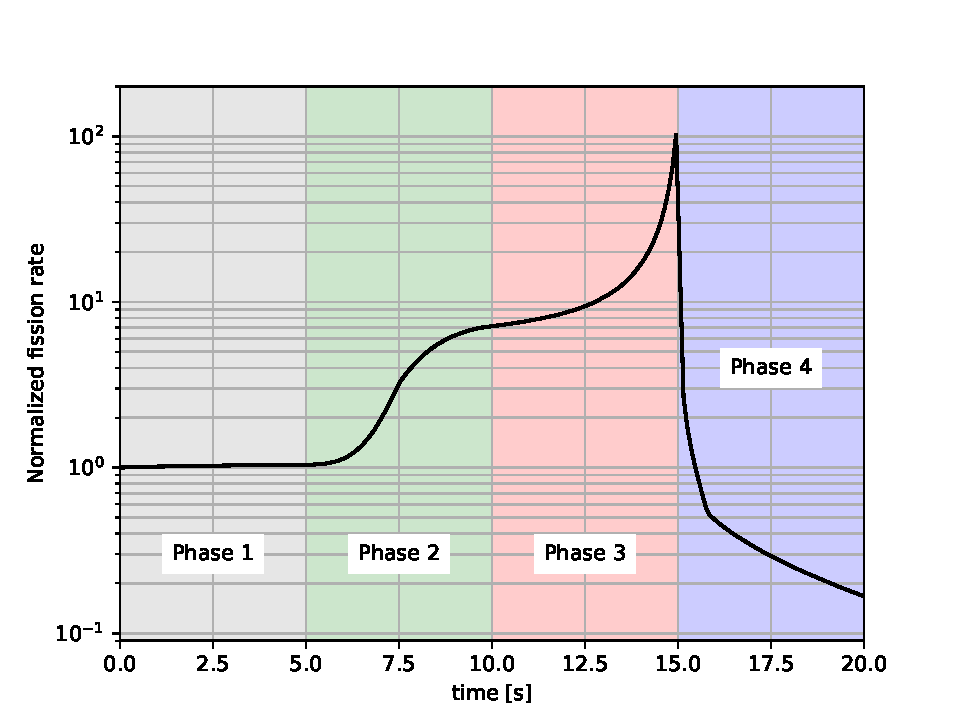
\includegraphics[width=0.48\linewidth]{figures/delta_figs/c5/acc.pdf}
    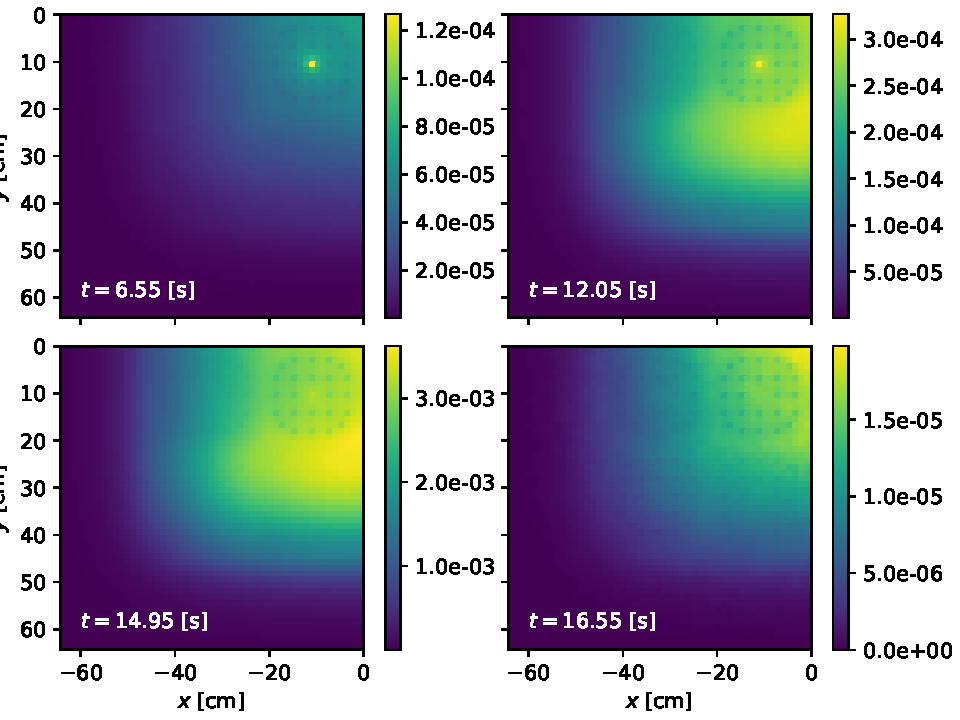
\includegraphics[width=0.48\linewidth]{figures/delta_figs/c5/flux.pdf}
    \caption{C5G7 stuck rod accident simulation, (left) flux densities through time, (right) scalar flux on x-y plane (top view) at points in time}
    \label{fig:c5g7}
\end{figure}

We first model this problem using the 7 group materials described by the normal C5G7 benchmark \cite{jia_hou_oecdnea_2017} which we will call C5G7 in the remainder of this work.
We model C5G7 with \num{3.9} million mesh cells in a full 3D, time and energy dependent tally mesh.
The movement of the control rods into and out of the reactor is controlled with MC/DC's continuous movement functionality.
To verify that the delta tracking methods we explore converge to the correct solutions while in transport with continuously moving surfaces we compare delta tracking solutions to solutions provided by surface tracking (which has already been verified and validated).
Performance data is collected by running \num{1e6} particles in \num{10} batches (total of \num{1e7} particles).

Next we define a continuous energy version of the C5G7 geometry we call C5CE undergoing the same four-phase accident.
Table \ref{tab:c5ce} in appendix \ref{app:c5ce_mat} shows material compositions for the C5CE problem.
Using this benchmark we evaluate both the voxelized tally method as well as the hybrid-in-energy method described in section \ref{sec:cutoff}.
Figure \ref{fig:majorant_c5ce} at right plots the macroscopic total and majorant cross sections over energy for the materials in C5CE.
The neutron resonances end around \SI{10}{\kilo\electronvolt} so we set a cut off at \SI{50}{\kilo\electronvolt}.
When running this problem particles moving at speeds above \SI{50}{\kilo\electronvolt} MC/DC will use voxelized Woodcock-delta tracking and blow it will use traditional surface tracking.
We expect this to provide significant speedup over all previous methods explored in this problem as we avoid both down falls of either tracking method (surface tracking moving from surface to surface and delta tracking getting stuck in the rejection sample). 
To quote Miley Cyrus, ``you get the best of both worlds" \cite{cyrus_best_2005}.
C5CE also includes the same continuously moving surfaces as C5G7 so it serves as an additional verification that delta tracking methods can be used in conjunction continuously moving surfaces.
We model this problem with \num{447} mesh tally bins in 2D $x$-$y$ geometry (integrated along $z$) time and energy dependent tally mesh.
We run \num{1e5} particles in a single batch.

% dragon intro
The next problem we consider is a full time-dependent simulation of the historical Dragon-burst experiments \cite{kimpland2021dragon}.
It was conducted in 1944 during the Manhattan project to prove that criticality could be achieved with prompt neutrons only.
Previous experiments, like the Chicago Pile One, used delayed neutrons to achieve criticality.
Figure \ref{fig:schems} at left shows a schematic of the experiment where a slug of highly enriched (75\%) Uranium Hydride ($UH_{10}$) was doped through a core with additional fuel.
As the slug moved through the core a prompt critical reaction was triggered as critical mass was achieved.
Before the super critical burst could become a problem (i.e., a deadly uncontrollable blast), gravity would pull the slug out of the core, ending the reaction.
Kimpland et. al showed that this burst criticality experiment could achieve over 9 orders of burst magnitude \cite{kimpland2021dragon}.
Work is on going to model the problem up to 9 orders of burst magnitude in MC/DC but here we use a less reactive version (25\% enrichment) to verify delta tracking with the hybrid-in-material method described in section \ref{sec:material_exc} and additional verification for delta tracking with continuously moving surfaces.
Figure \ref{fig:dragon_results} shows the overall flux density through time at left and a y-z plot of scalar flux at various points in time on the right.

\begin{figure}
    \centering
    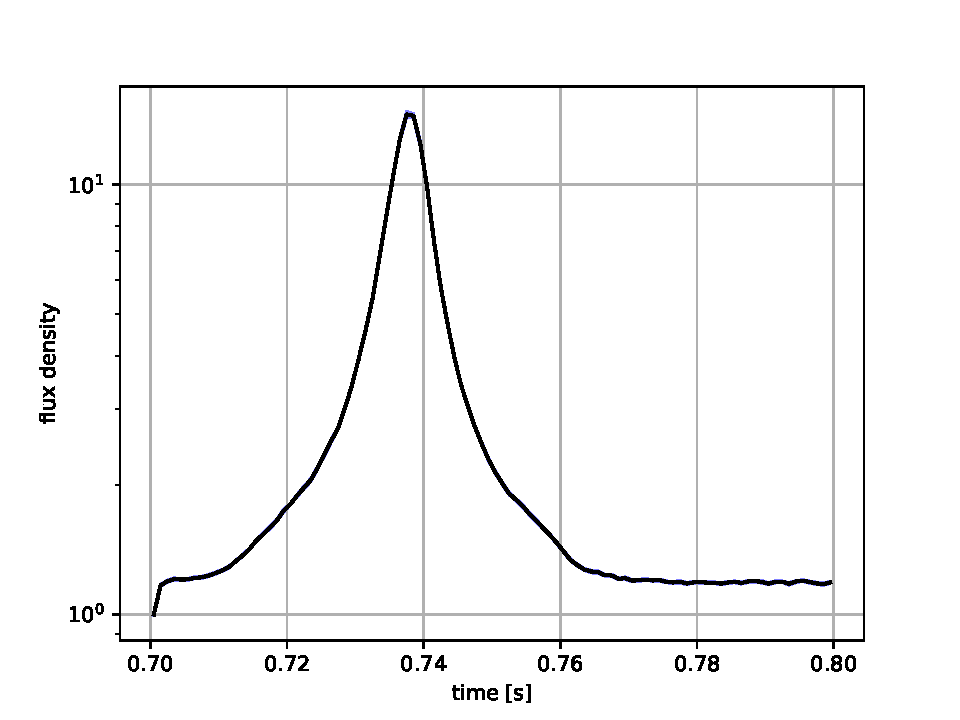
\includegraphics[width=0.48\linewidth]{figures/delta_figs/dragon/dragon_curve.pdf}
    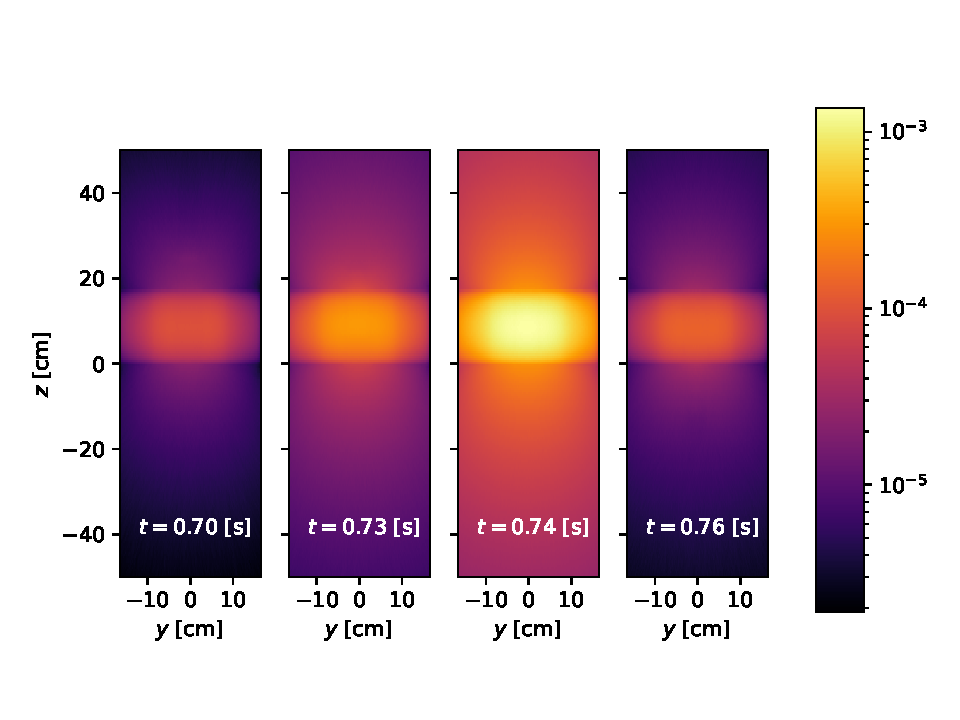
\includegraphics[width=0.48\linewidth]{figures/delta_figs/dragon/flux_dragon.pdf}
    \caption{Dragon burst simulation, (left) flux density through time, (right) scalar flux on y-z plane (side view) at points in time.}
    \label{fig:dragon_results}
\end{figure}

Figure \ref{fig:majorant_dragon} at left shows the continuous energy macroscopic total cross sections in the model we simulate.
The majorant, tamper and fuel cross sections all sit almost 4 orders magnitude above the cross section for air.
This is due to air being low density meaning fewer atoms for neutrons to interact with.
We expect any delta tracking algorithm to perform quite poorly in this model for a number of reasons.
First when undergoing delta tracking particles in the air region will get stuck in the rejection sample loop for a long time as the majorant is orders of magnitude larger and will sample very small distance before conducting a rejection sample.
Second as much of the problem is a void region the collision estimator that normal delta tracking requires will provide poor tallies in those regions
Third the problem is geometrically simple: consisting of a rectangular slug moving through a rectangular slab with a complimentary hole.
Traditional wisdom suggests that delta tracking performs best in complex materials.
The point of comparing delta tracking methods for this specific problem is to first confirm that delta tracking works with such a dynamic problem (the slug is modeled using MC/DC's continues movement functionality) and if we measure superior performance to standard delta tracking when using the hybrid-in-material method.

\section{Results}

% TLEase add the following required packages to your document preamble:
% \usepackage{multirow}
\begin{table}
\centering
\begin{tabular}{llllll}
\hline
Problem & Tracking Alg. & Estimator & Runtime [s] & $\left|\left|\hat{\sigma}^2\right|\right|_1$ & FOM \\ \hline
\multirow{4}{*}{Kobyashi}
 & surface  & TLE & \num{1574} & \num{4.514e-3} & 0.1407 \\
 & surface  & CE & \num{1014} & \num{9.552e-2} & 0.0103 \\
 & delta  & TLE & \num{1298} & \num{4.539e-3} & 0.1697 \\ 
 & delta  & CE & \num{817.2} & \num{2.062e-1}  & 0.0059 \\
 \hline
 

 
\multirow{4}{*}{C5G7}
 & surface  & TLE & \num{7926} & \num{1.295e-4} & \num{0.9744} \\
 & surface  & CE & \num{3173} & \num{1.295e-4} & \num{2.4336} \\
 & delta  & TLE & \num{2870.} & \num{1.400e-4} & \num{2.4889} \\
 & delta  & CE & \num{1820} & \num{2.152e-4} & \num{2.5515} \\
 \hline

 
\multirow{6}{*}{C5CE} 
 & surface  & TLE & \num{734.6} & \num{1.812e-3} & \num{0.7484}\\
 & surface  & CE & \num{587.8} & \num{1.812e-3} & \num{0.9391}\\
 & delta  & TLE & \num{496.8} & \num{4.906e-3} & \num{0.4103} \\
 & delta  & CE & \num{555.0} & \num{1.173e-2} &  \num{0.1536} \\
 & hybrid-energy & TLE & \num{226.25} & \num{1.164e-3} & \num{3.798} \\ 
 & hybrid-energy & CE & \num{220.5} & \num{1.144e-3} & \num{3.965} \\ 
 \hline

 
\multirow{4}{*}{Dragon} 
 & surface  & TLE & \num{3816} & \num{1.163e-6} & \num{221.4} \\
 & delta  & CE & DNF$^*$ & - & - \\
 & delta  & TLE & DNF$^*$ & - & - \\
 & hybrid-in-material & TLE & \num{15493} & \num{1.106e-6} & \num{58.40} \\
 \hline
\end{tabular}
\caption{Results for benchmark problems on Dane (112$\times$ Intel Sapphire Rapids CPU cores). $^*$Did not finish in 8 hour time limit.}
\label{tab:dane_results}
\end{table}

%1.163327654958653e-06
%1.1056932706381267e-06

% Please add the following required packages to your document preamble:
% \usepackage{multirow}
\begin{table}
\centering
\begin{tabular}{llllll}
\hline
Problem & Tracking Alg. & Estimator & Runtime [s] & $\left|\left|\hat{\sigma}^2\right|\right|_1$ & FOM \\ \hline
\multirow{4}{*}{Kobyashi} 
 & surface  & TLE & \num{973.9} & \num{4.514e-3} & 0.2275 \\
 & surface  & CE & \num{840.6} & \num{9.952e-2} & 0.0125 \\
 & delta  & TLE & \num{831.8} & \num{4.539e-3} & 0.2649 \\ 
 & delta  & CE & \num{620.7} & \num{2.062e-1}  & 0.0078 \\
 \hline
 
\multirow{4}{*}{C5G7} 
 & surface  & TLE & \num{4598} & \num{1.305e-4} & \num{1.666} \\
 & surface  & CE & \num{2403} & \num{1.305e-4} & \num{3.1878} \\
 & delta  & TLE & \num{1615} & \num{1.400e-4} & \num{4.4205} \\ 
 & delta  & CE & \num{789.3} & \num{2.152e-4} & \num{5.8860} \\
 \hline
 
\multirow{6}{*}{C5CE} 
 & surface  & TLE & \num{550.9} & \num{2.452e-3} & \num{0.7402}\\
 & surface  & CE & \num{465.9} & \num{2.452e-3} & \num{0.8753}\\
 & delta  & TLE & \num{500.7} & \num{1.690e-2} & \num{0.1182} \\
 & delta  & CE & \num{421.6} & \num{1.793e-2} &  \num{0.1323} \\
 & hybrid-energy & TLE & \num{291.7} & \num{1.557e-3} & \num{2.2023} \\ 
 & hybrid-energy & CE & \num{275.6} & \num{1.839e-3} & \num{1.9731} \\ 
 \hline
 
\multirow{4}{*}{Dragon} 
 & surface & TLE & \num{3993} & \num{1.163e-06} & \num{2153} \\
 & delta & CE & DNF$^*$ & - & - \\
 & delta & TLE & DNF$^*$ & - & - \\
 & hybrid-material & TLE & DNF$^*$ & - & - \\ \hline
\end{tabular}
\caption{Results for benchmark problems on Lassen (4$\times$ Nvidia Tesla V100). $^*$Did not finish in 8 hour time limit.}
\label{tab:lassen_results}
\end{table}

In this section we discuss performance results of the of the benchmarks described above with surface, traditional delta, voxelized delta tracking as well as the hybrid-in-energy and hybrid-in-material tracking algorithms.
In this section we also verify that the various delta tracking methods converge to the same solution as surface tracking while transporting on a geometry with continuously moving surfaces.

\subsection{Performance Results}

% testing systems
We ran our benchmark problems on high-performance computing systems available at Lawrence Livermore National Laboratory (LLNL): the Dane, and Lassen machines.
Dane is a CPU-only system with dual-socket Intel Xeon Sapphire Rapids CPUs, each with 56 cores for a total of 112 per node. 
Lassen is the open collaboration sibling to the Sierra machine with four Nvidia Tesla V100s GPUs and two IBM Power 9 CPUs per node.
We will make all performance statements against CPU runtime from a whole node of Dane (112 MPI threads, CPU) and a whole node of Lassen (4 MPI Threads, GPU).
We compile to Nvidia GPUs with CUDA v11.8 and
Nvida-PTX with Numba v0.59.0\footnote{Numba v0.59.1 is the most recent version to support Power9 CPUs}.
We compile to CPUs with Numba v0.60.0.
We build our delta tracking methods off of MC/DC v0.12.0 \cite{transport_cement_mcdc_2024} and compile with Harmonize v0.0.2 \cite{harmonize}.
We use double precision for all floating point operations.
% Introduce the table
Table \ref{tab:dane_results} and \ref{tab:lassen_results} show the wall-clock runtime, normalized standard deviations and figures of merit for our four benchmark problems from the Dane and Lassen machines respectively.

% Results Koby
The Kobyashi problem on Dane sees dramatic runtime improvements when moving from surface to delta tracking with a collision estimator.
However this does not make up for the two orders of magnitude additional variance on the tallies of interest.
This leads to a dramatically smaller figure of merit for traditional delta tracking (using a collision estimator) compared to surface tracking.
Figure \ref{fig:koby} shows the traditional delta tracking with a collision estimator on the bottom and our voxlized delta tracking on top at various points in time through the simulation.
It is clear to a casual observer that the collision estimator is producing a more variant (appearing as static-y or fuzzy) result than the track-length estimator.
Our voxlized tally method sees 21\% decrease in wall clock time compared with the same amount of normalized variance leading to a moderately improved figure of merit (\num{0.1697} and \num{0.1407} for our voxelized method and surface tracking respectively) 
This pattern of results, where traditional delta tracking is the fastest wall clock runtime with a normalized variance orders of magnitude above methods using a track-length estimator, will persist through the analysis of the other problems we consider.
As will the behavior of the voxelized delta method's runtime sitting between surface tracking and traditional delta tracking with similar variance to surface tracing results.


\begin{figure}
    \centering
    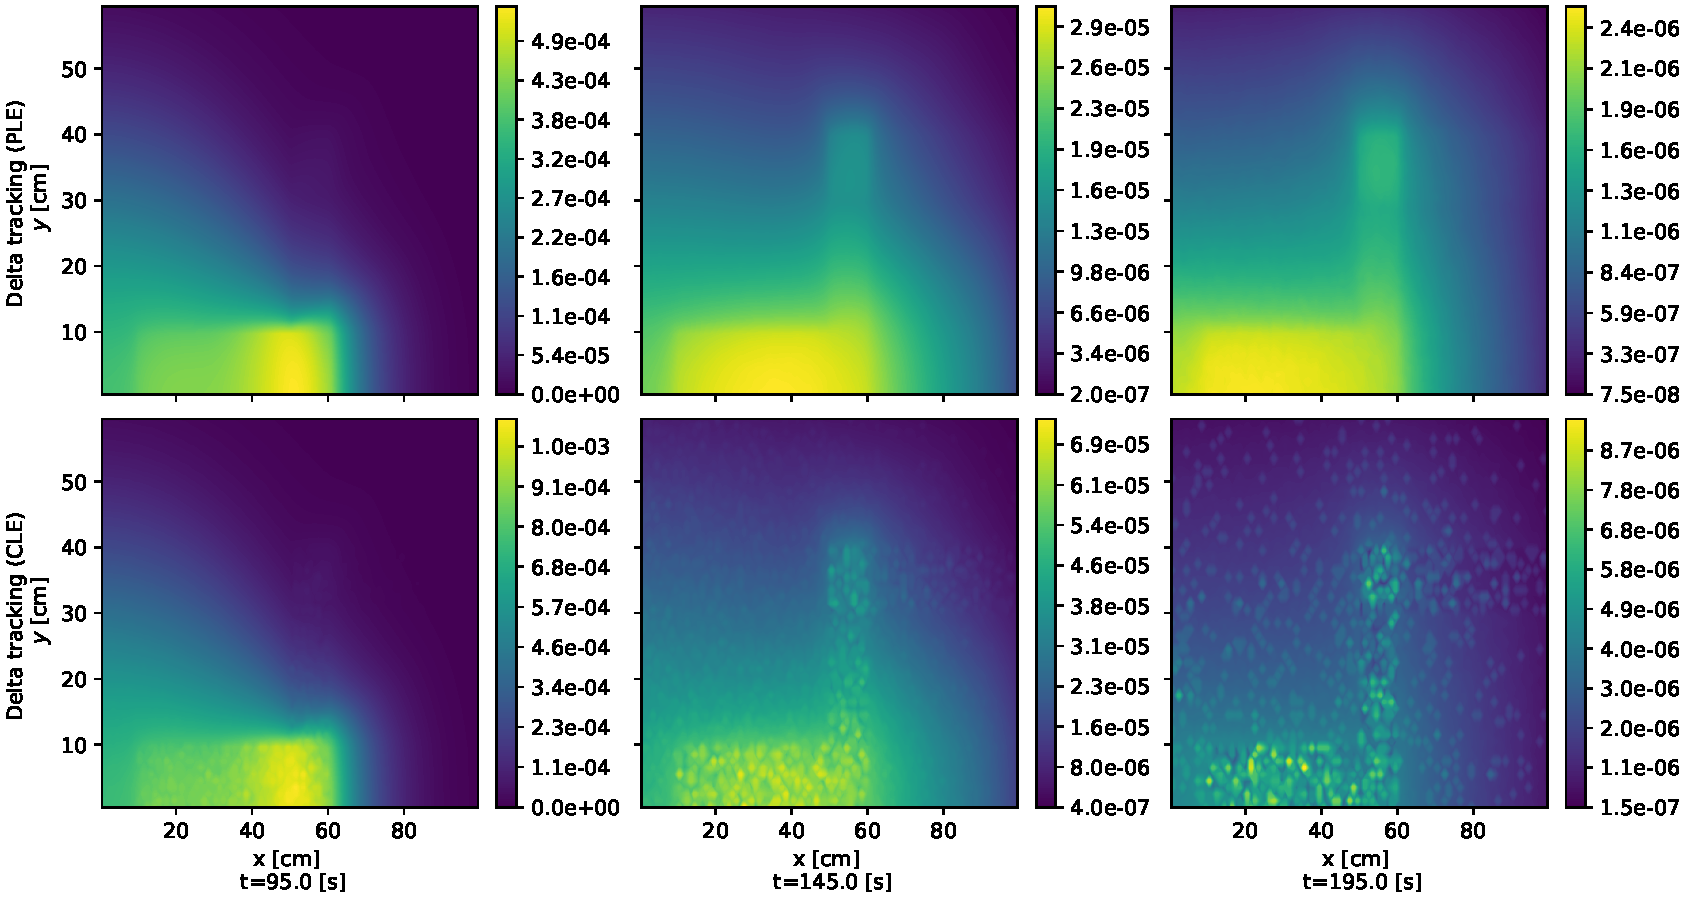
\includegraphics[width=\textwidth]{figures/delta_figs/cle_v_tle.pdf}
    \caption{Comparison of delta tracking using the track-length estimator (top row) and collision estimator (bottom row) at three points in time. Collision estimator has a much higher variance.}
    \label{fig:koby}
\end{figure}

% Restuls C5G7
Moving on to C5G7, the same pattern of results persists where traditional delta tracking sees the smallest wall-clock runtime with the highest variance (\SI{1673}{\s} and \num{0.20062} respectively), while surface tracking sees the longest runtime and voxelized delta tracking sits between the two (\SI{7920}{\s}, \SI{2870}{\s} respectively) with roughly the same error ($\approx$\num{1e-4}).
The pattern continues to persist on Lassen only with between \num{1.7}$\times$ and \num{2}$\times$ wall clock runtime speedup for all tracking methods when moving from Dane to Lassen while variance remains about the same.
Voxelized delta tracking shows a \num{2.6}$\times$ and \num{2.7}$\times$ higher figure of merit over surface tracking on Dane and Lassen respectively.

% Restuls C5CE
C5CE shows similar results to the previous benchmarks for surface traditional and voxelized tracking methods.
The speedup of Lassen over Dane is now lower (between \num{0.9}$\times$ and \num{1.3}$\times$ speedup) indicating improvements are needed for our continuous energy physics when implemented on GPU.
The hybrid-in-energy method sees the most significant improvement of figure of merit with an order of magnitude increase (\num{11}$\times$ on Dane \num{7}$\times$ on Lassen).


% Restuls Dragon
The performance of the Dragon problem is an outlier in the behavior of the methods we consider.
Delta tracking (both traditional and voxelized) do not finish on Dane or Lassen in the 8 hours given to complete the simulation on either machine.
As predicted the hybrid-in-material method does see improvement over the other two methods, as it completes the simulation in 4 hours while traditional surface tracking completes it in one.
Also as predicted this is a problem that does not warrant any delta tracking methods due to the material composition and geometric layout of the problem.
However, It further demonstrates that delta tracking methods can be used with the continuously moving surfaces implemented in MC/DC.


\section{Discussion, Conclusions, and Future Work}
\label{disucssions}

We have implemented, Woodcock-delta tracking in MC/DC on CPUs and GPUs including using a voxelized track-length tally to efficiently score integral track-length tallies while under going delta tracking.
We verify the solution produced by this method against various steady state and time-dependent anaclitic benchmark problems available in MC/DC's verification suite.
We also verify the Woodcock-delta tracking algorithm with the continuously moving surfaces in MC/DC using the fuel pellet problem.
We have shown figures of merit improve modestly in large scale multi-group and continuous energy time-dependent benchmark problems when using this tracking and tallying technique on CPUs and GPUs.

We have also demonstrated a novel hybrid surface-delta tracking scheme called hybrid-in-energy where surface and delta are used in low and high energies, respectively.
For a continuous energy version of the C5G7 benchmark geometry undergoing a four-phase accident we show an order of magnitude increase in figure of merit on both a CPU and GPU node.
We have also confirmed previously defined surface-hybrid delta tracking methods can produce better results in problems significant void regions \cite{leppanen_2010_burnup}.

A combination of a numerical method getting a lower variance with fewer particles and an efficient implementation of that numerical method.
Thus what makes a delta or surface tracking algorithm more ``efficient" than the other can vary code-to-code.
Not every code implements tallying the way MC/DC does meaning the added efficiency of using the voxelized tally 
This does make the repeatability of surface v delta tracking implementations less generalizable but this has been the case when confronting multiple developments in the Monte Carlo neutron transport space.
For example when implementing GPUs some production codes had relatively few algorithmic issues and substanital CS

The major take away of this work is that Delta and surface tracking do not have to be treated as discrete choices in numerical method.
Indeed this matches what the developers of Serpent2, and MONK/MCBEND have known for years.
Greater performance can be achieved by mixing and matching the underlying transport methods given the detectable physics of a simulation and the relative strengths and weakness of a given transport application.
As we discussed in section \ref{sec:implementation} taking a surface transport code and implementing delta tracking is simple given a method of computing a macroscopic majorant cross section.
This process has been completed at least twice now in MCATK \cite{morgan2023delta}, and MC/DC with work ongoing in OpenMC and MCNP. % cite their branch

For the voxelized tally method specifically this work is promising, but the lack of non-integral tallies means limited applicability to physical problems of interest.
Work is on-going in producing efficient methods of computing relevant macroscopic cross-sections defined on a structured mesh while a particle is undergoing transport.
This process is simple for multi-group cross-sections where reaction rates can be determined entirely as a post process but work is ongoing to identify the most efficient method for continuous energy transport.

A method of reducing the dimensionality of the majorant is also under active research in order to have a smaller more efficient majorant cross section lookup in the sample distance to collision operations.
Implementing post process reaction tallies for other quantities of interest
Experiments with the collision flux estimator and methods of tallying into vacuum and low interaction rate are being considered.
Research is also ongoing into methods to tallying with multiple estimators onto the same mesh.
If only one estimator is used at a time then we avoid the need for complex covariance computations (e.g., those implemented in MCNP \cite{urbatsch_estimation_1995} \cite{MCNP_RisingArmstrongEtAl}).

Combinations of the Woodcock-delta and surface tracking algorithms proves to be a compiling field of research in Monte Carlo neutron transport.
The combination of these two tracking algorithms allows for greater significances on a broader set of problem physics where one scheme may out perform another.
Either method is a valid sampling of the cumulative probability distribution function at any point in transport.
Modest to significant improvements may occor when taking advantage of that fact.


\section*{Acknowledgments}
We thank Patrick Shirwise and Paul Ramano of Argonne National Laboratory, Mike Rising of Los Alamos National Laboratory, Jaakko Leppänen of VTT Technical Research Center of Finland, and Simon Richards of ANSWERS software for productive conversations.
We also thank the high performance computing staff at Lawrence Livermore National Laboratory for continued support using the Dane machine. 

This work was supported by the Center for Exascale Monte-Carlo Neutron Transport (CEMeNT) a PSAAP-III project funded by the Department of Energy, grant number: DE-NA003967.

\section*{Appendix}


\subsection*{Continuous Energy Macroscopic Majorant}
\label{app:majorant}

To compute a unified energy grid per material we combine the energy grids from all nuclide in a given material. 
Then we call \texttt{numpy.unique()} which returns a sorted array (form smallest to largest) with no repeating elements \cite{van_der_walt_numpy_2011}.
To compute a unified energy grid for the whole problem we do the same but with all the nuclides in the entire problem.

Computing a macroscopic majorant for nuclides that are not on a unified energy grid requires two levels of interpolation to put a given macroscopic total cross section on a unified energy grid.
First interpolation from each nuclides microscopic cross section onto a materials unified energy grid to compute a macroscopic total cross section.
Then a second interpolation from the material to the majorant's unified energy grid.
We use \texttt{scipy.interpolate.interp1d()} to interpolate from one energy grid to the next \cite{2020SciPy-NMeth:a}. 

The following code shows exactly how this is done in MC/DC:

\begin{minted}[mathescape, linenos]{python}
import scipy
import numpy

# unify the energy grids from all nuclides
majorant_energy_grid = np.array([])
for n in range(N_nuclide):
    nuclide = mcdc["nuclides"][n]
    majorant_energy_grid = np.append(majorant_energy_grid, nuclide["E_xs"])

# sort energy grid and eliminate duplicate points
majorant_energy_grid = np.unique(majorant_energy_grid)
majorant_xsec = np.zeros_like(majorant_energy_grid)

for m in range(N_material):

    material = mcdc["materials"][m]

    material_energy_grid = np.array([])

    # copmute a unified energy grid across all nuclides of a given material
    for n in range(material["N_nuclide"]):
        nuclide = mcdc["nuclides"][n]
        material_energy_grid = np.append(
            material_energy_grid, nuclide["E_xs"]
        )
    material_energy_grid = np.unique(material_energy_grid)
    MacroXS = np.zeros_like(material_energy_grid)

    # compute the macroscopic total cross section of a material on its unified
    # energy grid
    for n in range(material["N_nuclide"]):
        ID_nuclide = material["nuclide_IDs"][n]
        nuclide = mcdc["nuclides"][ID_nuclide]

        # Get nuclide density
        N = material["nuclide_densities"][n]

        # putting the microscopic cross-sections on the unifed
        # material energy grid
        total_micro_xsec_unified = scipy.interpolate.interp1d(
            nuclide["E_xs"], nuclide["ce_total"], bounds_error=False
        )
        total_micro_xsec_unified = total_micro_xsec_unified(
            material_energy_grid
        )

        # Accumulate
        MacroXS += N * total_micro_xsec_unified

    # puting the total macroscopic cross sections on on the majorant energy grid
    total_xsec_unified = scipy.interpolate.interp1d(
        material_energy_grid, MacroXS, bounds_error=False
    )
    total_xsec_unified = total_xsec_unified(majorant_energy_grid)

    # compares old majorant xsec and the currently evaluated unified xsec 
    # and picks the larger xsecs
    majorant_xsec = np.max((majorant_xsec, total_xsec_unified), axis=0)

\end{minted}

This process results in a large majorant cross section that is quite unwieldy.
Other more efficient algorithms exist to produce a just as accurate majorant with fewer points.
Delta tracking codes like Serpent avoid the need for any of this by having all nuclides on a unified energy grid \cite{leppanen_2015_serpent}.

\newpage

\subsection*{C5CE Material Definition}
\label{app:c5ce_mat}
\begin{longtable}{|l|l|l|}
\hline
Material                         & Nuclide & Atom fraction          \\ \hline
\endfirsthead
%
\endhead
%
\multirow{5}{*}{UO2 Fuel}        & O-16     & \num{0.04585265389377734}    \\ \cline{2-3} 
                                 & O-17     & \num{1.7419604031574338e-05} \\ \cline{2-3} 
                                 & O-18     & \num{9.19424166352541e-05}   \\ \cline{2-3} 
                                 & U-235    & \num{0.0007217486041189947}  \\ \cline{2-3} 
                                 & U-238    & \num{0.02224950230720295}    \\ \hline
                                 & O-17     & \num{1.743649552488715e-05}  \\ \cline{2-3} 
\multirow{5}{*}{MOX-43 Fuel}     & O-16     & \num{0.04589711643122753}    \\ \cline{2-3} 
                                 & O-17     & \num{1.743649552488715e-05}  \\ \cline{2-3} 
                                 & O-18     & \num{9.203157163056531e-05}  \\ \cline{2-3} 
                                 & U-235    & \num{0.0003750264168772414}  \\ \cline{2-3} 
                                 & U-238    & \num{0.02262319599228636}    \\ \hline
\multirow{5}{*}{MOX-7 Fuel}      & O-16     & \num{0.04583036614158277}    \\ \cline{2-3} 
                                 & O-17     & \num{1.741113682662514e-05}  \\ \cline{2-3} 
                                 & O-18     & \num{9.189772587857765e-05}  \\ \cline{2-3} 
                                 & U-235    & \num{0.0005581382302893396}  \\ \cline{2-3} 
                                 & U-238    & \num{0.022404154012604437}   \\ \hline
\multirow{5}{*}{MOX-87 Fuel}     & O-16     & \num{0.04585265389377734}    \\ \cline{2-3} 
                                 & O-17     & \num{1.7419604031574338e-05} \\ \cline{2-3} 
                                 & O-18     & \num{9.19424166352541e-05}   \\ \cline{2-3} 
                                 & U-235    & \num{0.0007217486041189947}  \\ \cline{2-3} 
                                 & U-238    & \num{0.02224950230720295}    \\ \hline
\multirow{5}{*}{Guide Tube}      & H-1      & \num{0.050347844752850625}   \\ \cline{2-3} 
                                 & H-2      & \num{7.842394716362082e-06}  \\ \cline{2-3} 
                                 & O-16     & \num{0.025117935412784034}   \\ \cline{2-3} 
                                 & O-17     & \num{9.542402714463945e-06}  \\ \cline{2-3} 
                                 & O-18     & \num{5.03657582849965e-05}   \\ \hline
\multirow{5}{*}{Fission Chamber} & H-1      & \num{0.050347844752850625}   \\ \cline{2-3} 
                                 & H-2      & \num{7.842394716362082e-06}  \\ \cline{2-3} 
                                 & O-16     & \num{0.025117935412784034}   \\ \cline{2-3} 
                                 & O-17     & \num{9.542402714463945e-06}  \\ \cline{2-3} 
                                 & O-18     & \num{5.03657582849965e-05}   \\ \hline
\multirow{12}{*}{Control Rod}    & Ag-107   & \num{0.023523285675833942}   \\ \cline{2-3} 
                                 & Ag-109   & \num{0.02185429814297804}    \\ \cline{2-3} 
                                 & In-113   & \num{0.0003421922042655644}  \\ \cline{2-3} 
                                 & In-115   & \num{0.007651085167039375}   \\ \cline{2-3} 
                                 & Cd-106   & \num{3.38816276451386e-05}   \\ \cline{2-3} 
                                 & Cd-108   & \num{2.4166172970990425e-05} \\ \cline{2-3} 
                                 & Cd-110   & \num{0.0003393605596264083}  \\ \cline{2-3} 
                                 & Cd-111   & \num{0.0003482051612205208}  \\ \cline{2-3} 
                                 & Cd-112   & \num{0.0006561061533306398}  \\ \cline{2-3} 
                                 & Cd-113   & \num{0.00033274751904988726} \\ \cline{2-3} 
                                 & Cd-114   & \num{0.0007825159207295705}  \\ \cline{2-3} 
                                 & Cd-116   & \num{0.00020443276053837845} \\ \hline
\multirow{5}{*}{Moderator}       & H-1      & \num{0.050347844752850625}   \\ \cline{2-3} 
                                 & H-2      & \num{7.842394716362082e-06}  \\ \cline{2-3} 
                                 & O-16     & \num{0.025117935412784034}   \\ \cline{2-3} 
                                 & O-17     & \num{9.542402714463945e-06}  \\ \cline{2-3} 
                                 & O-18     & \num{5.03657582849965e-05}   \\ \hline
\caption{Materials used in C5CE problem}
\label{tab:c5ce}\\
\end{longtable}